In order to measure the performance of the different systems, the \textit{Equal Error Rate} metric
is chosen. As its name suggests, the \textit{EER} prioritizes in an equal manner the
\textit{false acceptance rate} and the \textit{false rejection rate}. This metric was used
in the previous works of the current line of investigation related to pronunciation assessment
at phone level \cite{detection_phone_level_mispronunciation_learning, main}, so the same approach
was taken in the present work.

% The process for evaluating the performance of the classifier goes as follows:
The process for evaluating the performance of a classifier usually involves the following steps:
At first, the decision function of the classifier, which can be for example predicted probabilities
or in our case distances to the hyperplane, is computed for each instance of the test set.
Then, the obtained results are used to generate
a distribution of the instances count as function of the values
in the domain of the decision function. Finally,
in order to make class predictions a threshold is chosen and the instances with a result of the
decision function above that threshold are classified as positive, while
those with results below the threshold are classified as negative. Most classifiers
usually set a threshold by default, such as 0 in the case of Support Vector Machines that
determines a separation of
positives and negative instances according to the sign of their distance to the hyperplane.

The EER can be found by sweeping the threshold until reaching the condition that
False Positive Rate (FPR) equals False Negative Rate (FNR). FPR is computed as
the number of negative instances wrongly categorized as positive: $\frac{FP}{TN+FP}$.
Analogously, FNR is computed as the number of positve instances wrongly categorized as negative:
$\frac{FN}{TP+FN}$. A simple example of EER threshold is
shown in Fig. \ref{fig:eer}.

\begin{figure}[H]
  \centering
  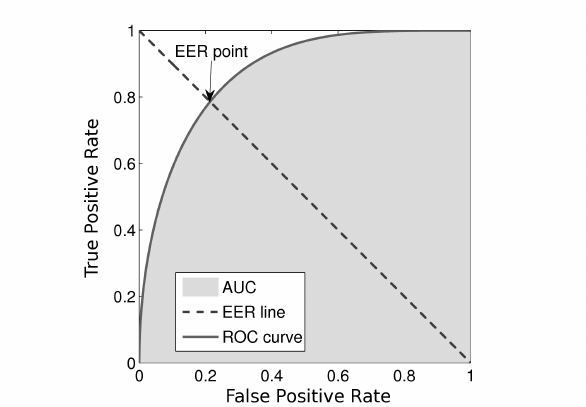
\includegraphics[width=0.8\textwidth]{files/figures/method/eer}
  \caption{An example of EER threshold with perfectly balanced classes. Both negative and positive distributions have the same size and shape.
  The threshold separates the instances in such way that FPR equals FNR.}
  \label{fig:eer}
\end{figure}

Even though the diagram shows a case where the classes are perfectly balanced, in most of
real world problems (including the current one) this does not happen. Distributions of both
classes usually differs in both size and shape. However,
as the technique is based on the \textit{rate} of misclassified positive and negative instances,
the EER method can be applied without any trouble for unbalanced datasets and
is computed exactly the same way: by sweeping the threshold until finding the point
where FPR equals FNR.


% \subsection{Receiving Operating Characteristic}

% The \textit{Receiving Operating Characteristic} (ROC) curve of a binary classifier is a plot
% that resumes information of how
% well a model can correctly detect positive instances at expenses of raising false alarms
% after being tested against a data set.

% When testing a given classifier on a dataset the results can be resumed in a particular table
% known as \textit{confusion matrix}:

% \begin{center}
%     \begin{tabular}{ | c | c | c | c | }
%     \hline
%     & \multicolumn{2}{  c | }{\textbf{Actual Class}} & \\ \hline
%     \textbf{Predicted Class} & \textit{Actual Positive} & \textit{Actual Negative} & \textit{Total Count} \\ \hline
%     \textit{Predicted Positive} & True Positive (TP) & False Positive (FP) & Total Positives (P) \\ \hline
%     \textit{Predicted Negative} & False Negative (FN) & True Negative (TN) & Total Negatives (N) \\ \hline
%     \end{tabular}
% \end{center}

% \textit{True Positive Rate} is calculated as the number of instances predicted
% as \textit{positive} which
% actually are \textit{positive} over the total number of \textit{positives} while
% \textit{False Positive Rate} is calculated as the number of instances predicted as
% \textit{positive} which actually are negative:

% \begin{multicols}{2}
%   \noindent
%   \begin{equation}
%     \label{eq:tpr}
%     TPR = \frac{TP}{P}
%   \end{equation}
%   \begin{equation}
%     \label{eq:fpr}
%     FPR = \frac{FP}{N}
%   \end{equation}
% \end{multicols}

% In a \textit{ROC} curve the \textit{TPR} is plotted in function of the \textit{FPR} for
% different cut-off points. Each point of the curve represents a {\textit{FPR},\textit{FPR}}
% pair corresponding to a particular decision threshold. A test with perfect discrimination
% (no overlap between the positives and negatives distributions) would have a \textit{ROC}
% curve that passes through the top left corner. So the closer the \textit{ROC} curve is to
% the upper left corner, the higher the overall accuracy of the test.

% \begin{figure}[H]
%   \centering
%   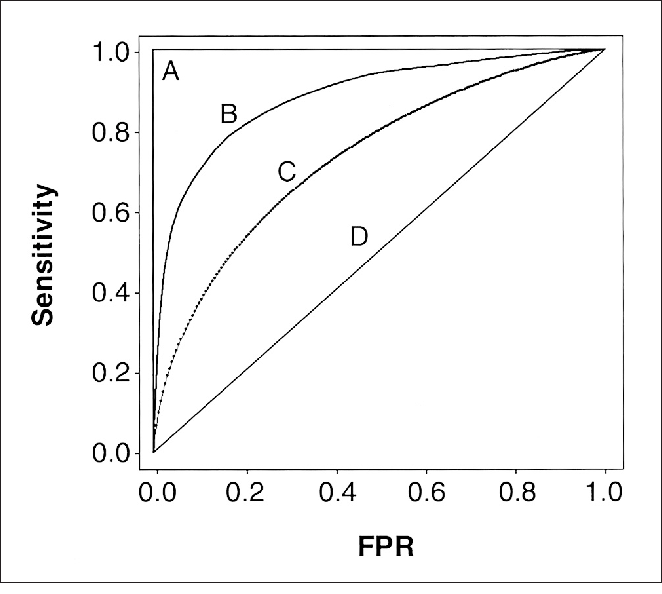
\includegraphics[width=0.5\textwidth]{files/figures/method/roc-curve}
%   \caption{ROC curve example. The closer the curve to the upper left corner, the higher the
%   accuracy of the system}
%   \label{fig:rocCurve}
% \end{figure}

% \subsection{Equal Error Rate}

% \textit{TPR} (Eq. \ref{eq:tpr}) is also called \textit{sensitivity} in the sense that measures
% the capacity of the system of detecting positive instances and classifying them
% correctly as positives.
% At the same time, \textit{specificity} is a measure of the capacity of the system of
% avoid raising false alarms, when classifiyng instances that actually belongs to the
% negative class. Or, in other words, the capacity of the system of detecting negative
% instances and classifying them correctly as negatives. \textit{FPR} (Eq. \ref{eq:fpr})
% is actually the complement of \textit{specificity}:

% \begin{equation}
% specificity = \frac{TN}{N} = \frac{TN}{TN+FP} = 1 - \frac{FP}{TN+FP} = 1 - FPR
% \end{equation}

% \textit{Equal Error Rate} (EER) is the value on which \textit{sensitivity} is equal to
% \textit{specificity}. At this point the system classifies correctly positive instances
% as well as it classifies negative instances, thus prioritizing both classes in the same
% way. It can be calculated easily as the point of intersection between the \textit{ROC}
% curve and the \textit{specificity} curve: $1-FPR$

% \begin{figure}[H]
%   \centering
%   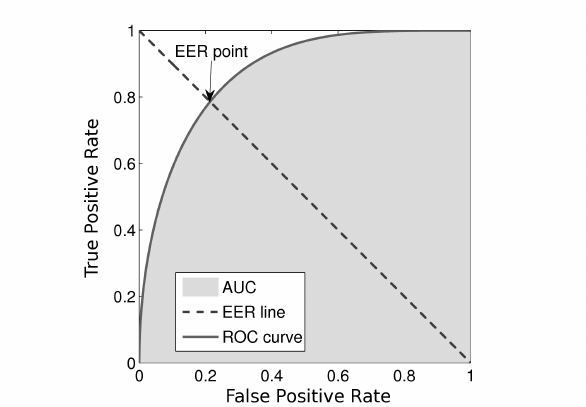
\includegraphics[width=0.5\textwidth]{files/figures/method/eer}
%   \caption{EER is equal to the value of the intersection between the ROC curve and
%   the Sensitivty curve as function of \textit{FPR}}
%   \label{fig:eer}
% \end{figure}

% \textit{EER} is a proper performance measure for the task of pronunciation assessment
% at phone level because both correctly pronounced and mispronounced
% classes are equally important. In other tasks, such as \textit{Bank Fraud} or
% \textit{Spam Detection}, it may be essential to strictly prioritize one class over the
% other. In the current task however it is reasonable to assign the same priority
% to both \textit{sensitivity} and \textit{specificity}.
% Anyway, it is worth mentioning that during language learning a student may get
% discouraged if she pronounces an utterance correctly and the system classifies her
% utterance as incorrect. A threshold can be chosen in order to ensure that
% a mispronunciation flag is raised only when the resulting score is above that
% threshold. The system could have made a mistake
% for instances labeled as incorrect with values below the threshold, so a conservative
% decision of not raising a mispronunciation flag can be taken to avoid discouraging
% the students.
